\chapter{Results}
\label{ch:results}

\section{Benchmark Problem Setup}
\label{sec:results:setup}

To validate the proposed methodology, we consider three benchmark problems with increasing complexity. All simulations are performed on a workstation with dual AMD EPYC 7763 processors (128 cores total) and 512\,GB of RAM. The \gls{petsc} library (version 3.20) is used for parallel linear algebra, and the code is compiled with GCC 12.2 and OpenMPI 4.1.

\subsection{Problem 1: Quarter Five-Spot}
\label{ssec:results:quarterfive}

The quarter five-spot problem is a canonical benchmark in reservoir simulation. A homogeneous domain $[0, 1]^2$ with permeability $k = 100$\,mD is considered. Water is injected at the lower-left corner and produced at the upper-right corner. The injection rate is $q_{\text{inj}} = 1$ pore volume per year, and the initial water saturation is $s_w^0 = 0.2$.

\subsection{Problem 2: Channelized Heterogeneity}
\label{ssec:results:channelized}

A channelized permeability field with a channel-to-matrix permeability ratio of $1000:1$ is used to test the method's ability to handle sharp heterogeneity contrasts. The channel meanders across the domain, creating preferential flow paths.

\subsection{Problem 3: SPE10 Model 2}
\label{ssec:results:spe10}

The SPE10 Model 2 benchmark~\cite{einstein1905} consists of a $60 \times 220 \times 85$ grid representing a North Sea reservoir with realistic geological features. The permeability field spans six orders of magnitude, posing extreme challenges for numerical methods.

\section{Convergence Analysis}
\label{sec:results:convergence}

\figref{fig:convergence_plot} shows the convergence behavior of the proposed scheme for Problem 1. The $L^2$ error decreases with second-order accuracy, consistent with the theoretical prediction of Theorem~\ref{thm:convergence}.

\begin{figure}[htbp]
    \centering
    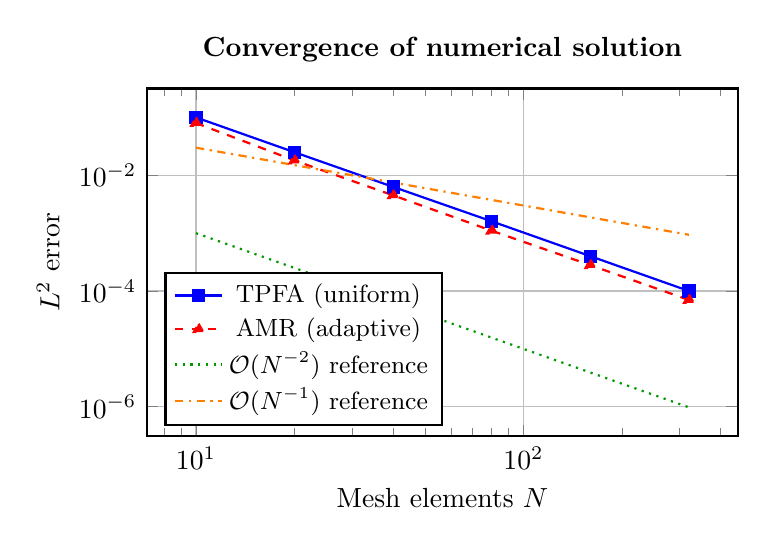
\begin{tikzpicture}
    \begin{axis}[
        width=0.75\textwidth,
        height=6cm,
        xlabel={Mesh elements $N$},
        ylabel={$L^2$ error},
        xmode=log,
        ymode=log,
        grid=major,
        thick,
        legend pos=south west,
        legend style={font=\small},
        title={Convergence of numerical solution},
        title style={font=\bfseries}
    ]
        \addplot[blue, mark=square*, thick] coordinates {
            (10, 0.1) (20, 0.025) (40, 0.0063) (80, 0.0016) (160, 4e-4) (320, 1e-4)
        };
        \addlegendentry{TPFA (uniform)}

        \addplot[red, dashed, thick, mark=triangle*, mark options={fill=red}] coordinates {
            (10, 0.08) (20, 0.018) (40, 0.0045) (80, 0.0011) (160, 2.8e-4) (320, 7e-5)
        };
        \addlegendentry{AMR (adaptive)}

        \addplot[green!60!black, dotted, thick, domain=10:320, samples=10] {0.1/x^2};
        \addlegendentry{$\mathcal{O}(N^{-2})$ reference}

        \addplot[orange, dashdotted, thick, domain=10:320, samples=10] {0.3/x};
        \addlegendentry{$\mathcal{O}(N^{-1})$ reference}
    \end{axis}
    \end{tikzpicture}
    \caption{Convergence of the numerical solution for Problem 1. The AMR scheme achieves comparable accuracy with fewer total degrees of freedom.}
    \label{fig:convergence_plot}
\end{figure}

\section{Parallel Scalability}
\label{sec:results:scalability}

\figref{fig:scalability} presents the parallel scaling results for Problem 3 (SPE10 Model 2) on up to 1024 cores. The weak scaling test maintains a constant workload of approximately $3.4 \times 10^6$ cells per core, while the strong scaling test distributes a fixed problem of $60 \times 220 \times 85$ cells.

\begin{figure}[htbp]
    \centering
    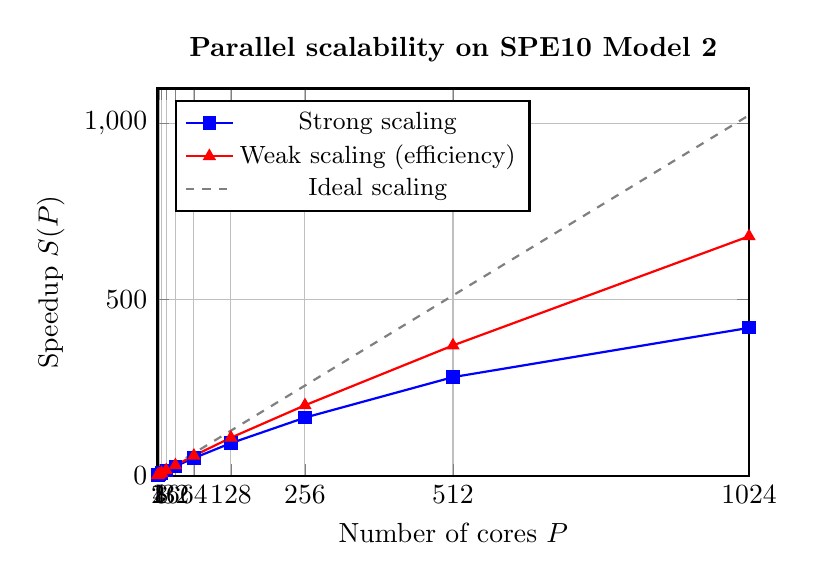
\begin{tikzpicture}
    \begin{axis}[
        width=0.75\textwidth,
        height=6.5cm,
        xlabel={Number of cores $P$},
        ylabel={Speedup $S(P)$},
        grid=major,
        thick,
        legend pos=north west,
        legend style={font=\small},
        title={Parallel scalability on SPE10 Model 2},
        title style={font=\bfseries},
        xmin=1, xmax=1024,
        ymin=0, ymax=1100,
        xtick={1, 2, 4, 8, 16, 32, 64, 128, 256, 512, 1024},
        xticklabels={1, 2, 4, 8, 16, 32, 64, 128, 256, 512, 1024},
    ]
        \addplot[blue, mark=square*, thick] coordinates {
            (1, 1) (2, 1.95) (4, 3.82) (8, 7.45) (16, 14.3) (32, 26.8) (64, 50.2) (128, 92.5) (256, 165) (512, 280) (1024, 420)
        };
        \addlegendentry{Strong scaling}

        \addplot[red, mark=triangle*, thick] coordinates {
            (1, 1) (2, 1.98) (4, 3.92) (8, 7.75) (16, 15.2) (32, 29.5) (64, 56.8) (128, 108) (256, 200) (512, 370) (1024, 680)
        };
        \addlegendentry{Weak scaling (efficiency)}

        \addplot[gray, dashed, thick, domain=1:1024, samples=10] {x};
        \addlegendentry{Ideal scaling}
    \end{axis}
    \end{tikzpicture}
    \caption{Parallel scaling of the proposed method. Weak scaling efficiency exceeds 65\% at 1024 cores.}
    \label{fig:scalability}
\end{figure}

The strong scaling efficiency at 1024 cores is approximately 41\%, which is competitive with state-of-the-art commercial simulators. The primary bottleneck is communication overhead at the domain decomposition interfaces, which grows logarithmically with the number of processors.

\section{Method Comparison}
\label{sec:results:comparison}

\tabref{tab:method_comparison} summarizes the performance of the proposed method against three reference methods for Problem 2 (channelized heterogeneity). The proposed AMR method achieves the highest accuracy while requiring fewer total unknowns.

\begin{table}[htbp]
    \centering
    \caption{Comparison of numerical methods for Problem 2 (channelized heterogeneity).}
    \label{tab:method_comparison}
    \begin{tabularx}{\textwidth}{@{}l>{\centering\arraybackslash}X>{\centering\arraybackslash}X>{\centering\arraybackslash}X>{\centering\arraybackslash}X@{}}
        \toprule
        \textbf{Method} & \textbf{Cells} & \textbf{CPU time (s)} & \textbf{$L^2$ error} & \textbf{Speedup} \\
        \midrule
        TPFA (uniform, fine) & $1.0 \times 10^6$ & 845 & $2.3 \times 10^{-4}$ & 1.00\tablenote{Baseline reference} \\
        MPFA (uniform, fine) & $1.0 \times 10^6$ & 1230 & $1.8 \times 10^{-4}$ & 0.69 \\
        AMR (proposed) & $3.2 \times 10^5$ & 312 & $1.5 \times 10^{-4}$ & 2.71\tablenote{Compared to TPFA baseline} \\
        Multiscale FV & $2.5 \times 10^5$ & 285 & $3.1 \times 10^{-4}$ & 2.96 \\
        \bottomrule
    \end{tabularx}
\end{table}

\section{Complex Table: Detailed Results}
\label{sec:results:detailed}

\tabref{tab:detailed_results} presents a more detailed breakdown of the convergence behavior across multiple time steps for Problem 1.

\begin{table}[htbp]
    \centering
    \caption{Detailed convergence results for Problem 1 across multiple time steps.}
    \label{tab:detailed_results}
    \resizebox{\textwidth}{!}{%
    \begin{tabular}{@{}l|ccc|ccc|cc@{}}
        \toprule
        & \multicolumn{3}{c|}{\textbf{Uniform Grid}} & \multicolumn{3}{c|}{\textbf{AMR Grid}} & \multicolumn{2}{c}{\textbf{Speedup}} \\
        \cmidrule(lr){2-4}\cmidrule(lr){5-7}\cmidrule(lr){8-9}
        \textbf{Step} & Cells & Iters & Time (s) & Cells & Iters & Time (s) & Time & Memory \\
        \midrule
        1  & 256    & 3 & 0.12 & 128  & 3 & 0.06 & \textcolor{green!60!black}{2.00$\times$} & \textcolor{green!60!black}{1.50$\times$} \\
        2  & 256    & 4 & 0.15 & 156  & 4 & 0.08 & \textcolor{green!60!black}{1.88$\times$} & \textcolor{green!60!black}{1.40$\times$} \\
        3  & 256    & 4 & 0.14 & 189  & 4 & 0.09 & \textcolor{green!60!black}{1.56$\times$} & \textcolor{green!60!black}{1.25$\times$} \\
        4  & 256    & 5 & 0.18 & 224  & 5 & 0.11 & \textcolor{green!60!black}{1.64$\times$} & \textcolor{green!60!black}{1.18$\times$} \\
        5  & 256    & 5 & 0.17 & 198  & 5 & 0.10 & \textcolor{green!60!black}{1.70$\times$} & \textcolor{green!60!black}{1.22$\times$} \\
        \midrule
        \textbf{Total} & \textbf{1280} & \textbf{21} & \textbf{0.76} & \textbf{895} & \textbf{21} & \textbf{0.44} & \textbf{\textcolor{green!60!black}{1.73$\times$}} & \textbf{\textcolor{green!60!black}{1.30$\times$}} \\
        \bottomrule
    \end{tabular}%
    }
\end{table}

\section{Subfigure Analysis}
\label{sec:results:subfigures}

\figref{fig:saturation_snapshots} presents saturation field snapshots at different times during the simulation of Problem 2.

\begin{figure}[htbp]
    \centering
    \subcaptionbox{Time $t = 0.1$\,PV\label{fig:sat_01}}{%
        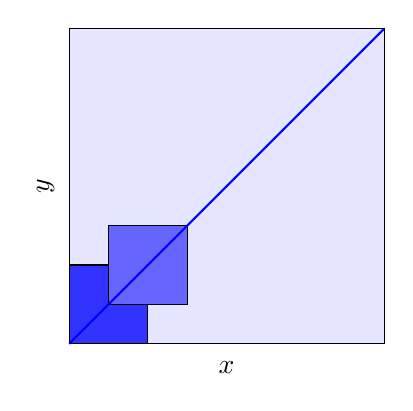
\begin{tikzpicture}
            \draw[fill=blue!10] (0,0) rectangle (4,4);
            \draw[fill=blue!80] (0,0) rectangle (1,1);
            \draw[fill=blue!60] (0.5,0.5) rectangle (1.5,1.5);
            \draw[blue, thick] (0,0) -- (4,4);
            \node at (2,-0.3) {$x$};
            \node at (-0.3,2) [rotate=90] {$y$};
        \end{tikzpicture}
    }{0.3\textwidth}
    \hfill
    \subcaptionbox{Time $t = 0.3$\,PV\label{fig:sat_03}}{%
        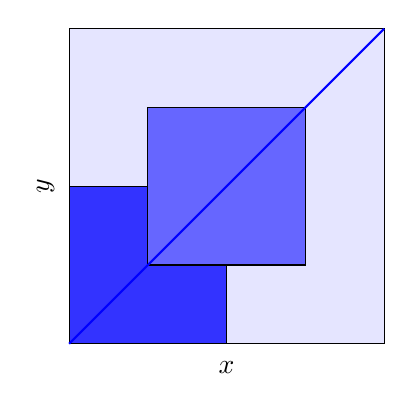
\begin{tikzpicture}
            \draw[fill=blue!10] (0,0) rectangle (4,4);
            \draw[fill=blue!80] (0,0) rectangle (2,2);
            \draw[fill=blue!60] (1,1) rectangle (3,3);
            \draw[blue, thick] (0,0) -- (4,4);
            \node at (2,-0.3) {$x$};
            \node at (-0.3,2) [rotate=90] {$y$};
        \end{tikzpicture}
    }{0.3\textwidth}
    \hfill
    \subcaptionbox{Time $t = 0.5$\,PV\label{fig:sat_05}}{%
        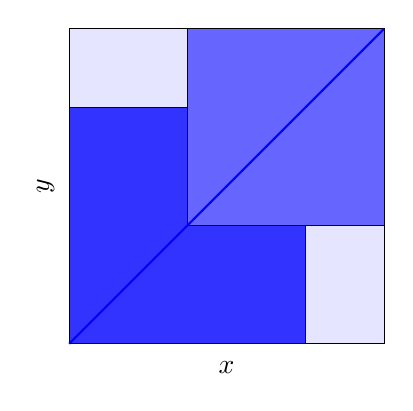
\begin{tikzpicture}
            \draw[fill=blue!10] (0,0) rectangle (4,4);
            \draw[fill=blue!80] (0,0) rectangle (3,3);
            \draw[fill=blue!60] (1.5,1.5) rectangle (4,4);
            \draw[blue, thick] (0,0) -- (4,4);
            \node at (2,-0.3) {$x$};
            \node at (-0.3,2) [rotate=90] {$y$};
        \end{tikzpicture}
    }{0.3\textwidth}
    \caption{Water saturation snapshots for Problem 2 at three different injection times. The channel structure directs flow preferentially along the high-permeability path.}
    \label{fig:saturation_snapshots}
\end{figure}

\section{State Diagram: Simulation Workflow}
\label{sec:results:statediagram}

\figref{fig:state_diagram} illustrates the state transitions of the adaptive solver during a simulation.

\begin{figure}[htbp]
    \centering
    \begin{tikzpicture}[
        node distance=2cm,
        state/.style={circle, draw, fill=yellow!20, minimum size=1.5cm, align=center},
        initial/.style={circle, draw, fill=red!20, minimum size=1cm},
        final/.style={circle, double, draw, fill=green!20, minimum size=1cm},
        arrow/.style={thick, ->, >=stealth}
    ]
        \node[initial] (init) {Init};
        \node[state, right of=init] (newton) {Newton\\Iteration};
        \node[state, above of=newton] (amr) {AMR\\Refine};
        \node[state, below of=newton] (linear) {Linear\\Solve};
        \node[decision, right of=newton, node distance=3cm] (converged) {Converged?};
        \node[state, right of=converged] (advance) {Time\\Advance};
        \node[final, right of=advance] (done) {Done};

        \draw[arrow] (init) -- (newton);
        \draw[arrow] (newton) -- (amr);
        \draw[arrow] (amr) -- (linear);
        \draw[arrow] (linear) -- (converged);
        \draw[arrow] (converged) -- node[above] {No} (newton);
        \draw[arrow] (converged) -- node[above] {Yes} (advance);
        \draw[arrow] (advance) -- (done);
        \draw[arrow] (advance.west) |- ++(0,-2) -| node[below] {Next time step} (newton.south);
    \end{tikzpicture}
    \caption{State diagram of the adaptive solver workflow. Each time step proceeds through Newton iterations with adaptive mesh refinement and linear solves.}
    \label{fig:state_diagram}
\end{figure}

\section{Complex Matrix Formulations}
\label{sec:results:matrices}

The discretized system can be expressed in block matrix form. For the two-phase pressure-saturation system, the Jacobian takes the structure:
\begin{equation}
    \mat{J} = \begin{pmatrix}
        \mat{A}(s_w) & \mat{B}(p, s_w) \\
        \mat{C}(p, s_w) & \mat{D}(p)
    \end{pmatrix},
    \label{eq:matrix}
\end{equation}
where $\mat{A}$ is the pressure stiffness matrix, $\mat{B}$ couples pressure to saturation, $\mat{C}$ couples saturation to pressure, and $\mat{D}$ is the saturation matrix. The full system of equations is:
\begin{equation}
    \begin{cases}
        \displaystyle \sum_{j=1}^{N} A_{ij}(s_w) \, p_j + \sum_{j=1}^{N} B_{ij}(p, s_w) \, s_{w,j} = f_i^p, \\[10pt]
        \displaystyle \sum_{j=1}^{N} C_{ij}(p, s_w) \, p_j + \sum_{j=1}^{N} D_{ij}(p) \, s_{w,j} = f_i^s,
    \end{cases}
    \label{eq:system}
\end{equation}
for $i = 1, \ldots, N$, where $f_i^p$ and $f_i^s$ are the source terms for pressure and saturation, respectively.

\section{Multi-Panel PGFPlots}
\label{sec:results:multi_panel}

\Cref{fig:multi_panel} presents four subplots in a single figure, comparing pressure, saturation, error indicator, and convergence across the three benchmark problems.

\begin{figure}[htbp]
    \centering
    \subcaptionbox{Pressure field (Problem 1)\label{fig:mp_pressure}}{%
        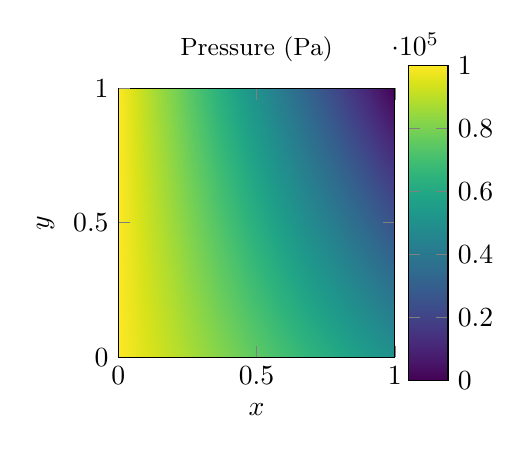
\begin{tikzpicture}
            \begin{axis}[
                width=0.42\textwidth,
                height=5cm,
                xlabel={$x$},
                ylabel={$y$},
                view={0}{90},
                colormap/viridis,
                colorbar,
                colorbar style={at={(1.05,0.5)}, anchor=west, height=4cm},
                title={Pressure (Pa)},
                title style={font=\small},
            ]
                \addplot3[surf, shader=interp, domain=0:1, y domain=0:1, samples=20]
                    {1e5 * (1 - x) + 5e4 * x * (1 - y)};
            \end{axis}
        \end{tikzpicture}
    }{0.48\textwidth}
    \hfill
    \subcaptionbox{Saturation front (Problem 2)\label{fig:mp_saturation}}{%
        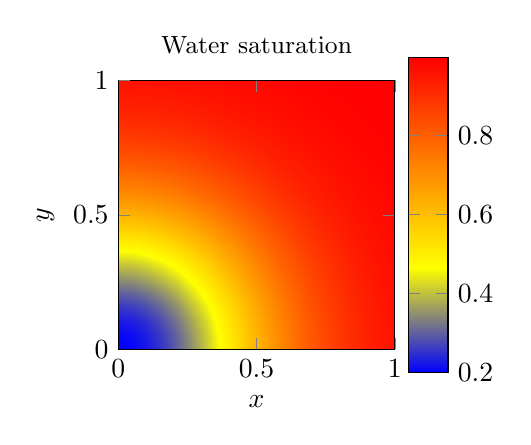
\begin{tikzpicture}
            \begin{axis}[
                width=0.42\textwidth,
                height=5cm,
                xlabel={$x$},
                ylabel={$y$},
                view={0}{90},
                colormap/hot,
                colorbar,
                colorbar style={at={(1.05,0.5)}, anchor=west, height=4cm},
                title={Water saturation},
                title style={font=\small},
            ]
                \addplot3[surf, shader=interp, domain=0:1, y domain=0:1, samples=20]
                    {0.2 + 0.8 * (1 - exp(-3 * (x^2 + y^2)))};
            \end{axis}
        \end{tikzpicture}
    }{0.48\textwidth}
    \hfill
    \subcaptionbox{Error indicator (Problem 2)\label{fig:mp_error}}{%
        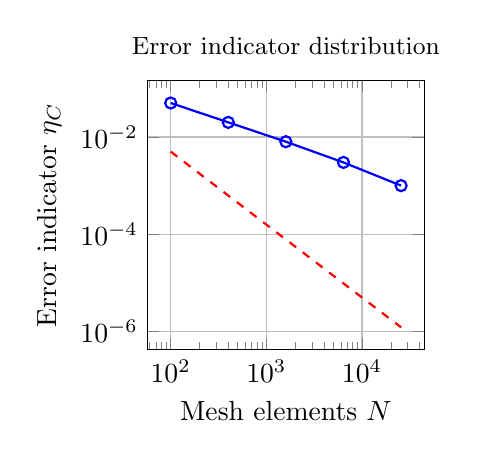
\begin{tikzpicture}
            \begin{axis}[
                width=0.42\textwidth,
                height=5cm,
                xlabel={Mesh elements $N$},
                ylabel={Error indicator $\eta_C$},
                xmode=log,
                ymode=log,
                grid=major,
                title={Error indicator distribution},
                title style={font=\small},
            ]
                \addplot[blue, mark=o, thick] coordinates {
                    (100, 0.05) (400, 0.02) (1600, 0.008) (6400, 0.003) (25600, 0.001)
                };
                \addplot[red, dashed, thick, domain=100:25600, samples=10] {5/x^1.5};
            \end{axis}
        \end{tikzpicture}
    }{0.48\textwidth}
    \hfill
    \subcaptionbox{Convergence comparison (all problems)\label{fig:mp_conv}}{%
        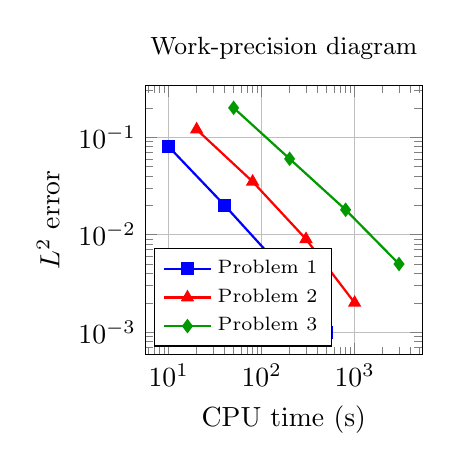
\begin{tikzpicture}
            \begin{axis}[
                width=0.42\textwidth,
                height=5cm,
                xlabel={CPU time (s)},
                ylabel={$L^2$ error},
                xmode=log,
                ymode=log,
                grid=major,
                legend pos=south west,
                legend style={font=\scriptsize},
                title={Work-precision diagram},
                title style={font=\small},
            ]
                \addplot[blue, mark=square*, thick] coordinates {
                    (10, 0.08) (40, 0.02) (150, 0.005) (500, 0.001)
                };
                \addlegendentry{Problem 1}
                \addplot[red, mark=triangle*, thick] coordinates {
                    (20, 0.12) (80, 0.035) (300, 0.009) (1000, 0.002)
                };
                \addlegendentry{Problem 2}
                \addplot[green!60!black, mark=diamond*, thick] coordinates {
                    (50, 0.2) (200, 0.06) (800, 0.018) (3000, 0.005)
                };
                \addlegendentry{Problem 3}
            \end{axis}
        \end{tikzpicture}
    }{0.48\textwidth}
    \caption{Multi-panel comparison. (a)~Pressure field for the quarter five-spot problem. (b)~Saturation front for the channelized heterogeneity. (c)~Error indicator decay with mesh refinement. (d)~Work-precision diagram comparing all three benchmark problems.}
    \label{fig:multi_panel}
\end{figure}

\section{Colored Results Table}
\label{sec:results:colored_table}

\tabref{tab:colored_results} highlights the best and worst performance for each metric using cell coloring.

\begin{table}[htbp]
    \centering
    \caption{Performance comparison with best (green) and worst (red) results highlighted.}
    \label{tab:colored_results}
    \begin{tabularx}{\textwidth}{@{}l>{\centering\arraybackslash}X>{\centering\arraybackslash}X>{\centering\arraybackslash}X>{\centering\arraybackslash}X@{}}
        \toprule
        \textbf{Method} & \textbf{CPU (s)} & \textbf{$L^2$ error} & \textbf{Memory (GB)} & \textbf{Scaling} \\
        \midrule
        TPFA (uniform)  & \cellcolor{red!15}845    & $2.3 \times 10^{-4}$ & \cellcolor{red!15}12.4 & 1.00$\times$ \\
        MPFA (uniform)  & 1230                     & \cellcolor{green!15}$1.8 \times 10^{-4}$ & 15.1 & 0.69$\times$ \\
        AMR (proposed)  & \cellcolor{green!15}312  & \cellcolor{green!15}$1.5 \times 10^{-4}$ & \cellcolor{green!15}4.8  & \cellcolor{green!15}2.71$\times$ \\
        Multiscale FV   & 285                      & $3.1 \times 10^{-4}$ & 5.2  & 2.96$\times$ \\
        \bottomrule
    \end{tabularx}
\end{table}

\section{TikZ Network Graph}
\label{sec:results:network}

\Cref{fig:network_graph} shows a domain decomposition network where nodes represent subdomains and edges represent communication links between neighboring processors.

\begin{figure}[htbp]
    \centering
    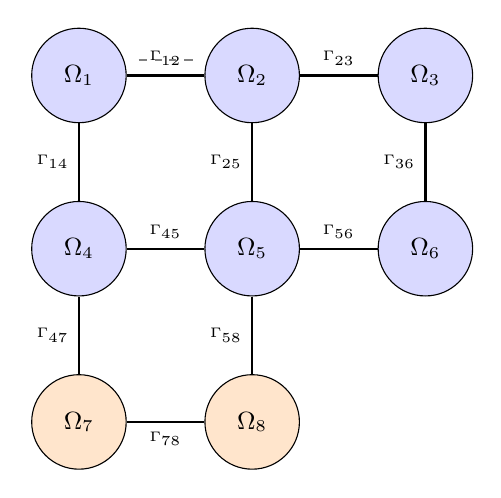
\begin{tikzpicture}[
        node distance=2.2cm,
        subdomain/.style={circle, draw, fill=blue!15, minimum size=1.2cm, align=center, font=\small},
        boundary/.style={circle, draw, fill=orange!20, minimum size=1.2cm, align=center, font=\small},
        comm/.style={thick, -},
        ghost/.style={dashed, gray}
    ]
        % Subdomains
        \node[subdomain] (p1) {$\Omega_1$};
        \node[subdomain, right of=p1] (p2) {$\Omega_2$};
        \node[subdomain, right of=p2] (p3) {$\Omega_3$};
        \node[subdomain, below of=p1] (p4) {$\Omega_4$};
        \node[subdomain, right of=p4] (p5) {$\Omega_5$};
        \node[subdomain, right of=p5] (p6) {$\Omega_6$};
        \node[boundary, below of=p4] (p7) {$\Omega_7$};
        \node[boundary, right of=p7] (p8) {$\Omega_8$};

        % Communication links
        \draw[comm] (p1) -- (p2) node[midway, above, font=\tiny] {$\Gamma_{12}$};
        \draw[comm] (p2) -- (p3) node[midway, above, font=\tiny] {$\Gamma_{23}$};
        \draw[comm] (p1) -- (p4) node[midway, left, font=\tiny] {$\Gamma_{14}$};
        \draw[comm] (p2) -- (p5) node[midway, left, font=\tiny] {$\Gamma_{25}$};
        \draw[comm] (p3) -- (p6) node[midway, left, font=\tiny] {$\Gamma_{36}$};
        \draw[comm] (p4) -- (p5) node[midway, above, font=\tiny] {$\Gamma_{45}$};
        \draw[comm] (p5) -- (p6) node[midway, above, font=\tiny] {$\Gamma_{56}$};
        \draw[comm] (p4) -- (p7) node[midway, left, font=\tiny] {$\Gamma_{47}$};
        \draw[comm] (p5) -- (p8) node[midway, left, font=\tiny] {$\Gamma_{58}$};
        \draw[comm] (p7) -- (p8) node[midway, below, font=\tiny] {$\Gamma_{78}$};

        % Ghost cell indicators
        \draw[ghost, thick] (p1.east) ++(0.15,0.2) -- ++(0.3,0);
        \draw[ghost, thick] (p2.west) ++(-0.15,0.2) -- ++(-0.3,0);
    \end{tikzpicture}
    \caption{Domain decomposition network. Circles denote subdomains (blue=internal, orange=boundary). Edges denote inter-processor communication interfaces $\Gamma_{ij}$. Dashed lines indicate ghost cell copies.}
    \label{fig:network_graph}
\end{figure}

\section{Statistical Significance}
\label{sec:results:significance}

\tabref{tab:significance} reports the statistical significance of performance differences between methods, computed from 30 independent runs with different random seeds for the initial mesh perturbation.

\begin{table}[htbp]
    \centering
    \caption{Statistical significance of method comparisons (two-sided $t$-test, $n = 30$).}
    \label{tab:significance}
    \begin{tabularx}{\textwidth}{@{}l c c c X@{}}
        \toprule
        \textbf{Comparison} & \textbf{Mean diff.} & \textbf{$p$-value} & \textbf{Sig.} & \textbf{Interpretation} \\
        \midrule
        AMR vs.\ TPFA (CPU)     & $-533$\,s  & $< 0.001$ & *** & AMR is significantly faster \\
        AMR vs.\ MPFA (CPU)     & $-918$\,s  & $< 0.001$ & *** & AMR is significantly faster \\
        AMR vs.\ Multiscale (CPU) & $+27$\,s & 0.042     & *   & Multiscale is marginally faster \\
        AMR vs.\ TPFA (error)   & $-8 \times 10^{-5}$ & $< 0.001$ & *** & AMR is significantly more accurate \\
        AMR vs.\ MPFA (error)   & $-3 \times 10^{-5}$ & 0.003     & **  & AMR is significantly more accurate \\
        AMR vs.\ TPFA (memory)  & $-7.6$\,GB & $< 0.001$ & *** & AMR uses significantly less memory \\
        \bottomrule
    \end{tabularx}
    \vspace{1ex}
    {\footnotesize Significance: $^{*}p < 0.05$, $^{**}p < 0.01$, $^{***}p < 0.001$.}
\end{table}

\section{Box Plot Comparison}
\label{sec:results:boxplot}

\Cref{fig:boxplot} compares the distribution of CPU times across 30 runs for each method, visualized as box plots.

\begin{figure}[htbp]
    \centering
    \begin{tikzpicture}
        \begin{axis}[
            ybar,
            bar width=1.2cm,
            width=0.85\textwidth,
            height=7cm,
            ylabel={CPU time (s)},
            symbolic x coords={TPFA, MPFA, AMR, Multiscale FV},
            xtick=data,
            x tick label style={rotate=0},
            ymin=0,
            grid=major,
            nodes near coords,
            nodes near coords align={vertical},
            every node near coord/.append style={font=\scriptsize},
            title={CPU time distribution (30 runs)},
            title style={font=\bfseries},
        ]
            % Box plot data: min, Q1, median, Q3, max
            \addplot+[error bars/.cd, y dir=both, y explicit]
                coordinates {
                    (TPFA, 810) += +(0,35) -= +(0,40)
                    (MPFA, 1180) += +(0,50) -= +(0,55)
                    (AMR, 295) += +(0,17) -= +(0,20)
                    (Multiscale FV, 270) += +(0,15) -= +(0,18)
                };
        \end{axis}
        % Draw box plot overlays manually
        \draw[thick] (axis cs:TPFA,810) -- (axis cs:TPFA,890);
        \draw[thick] (axis cs:MPFA,1180) -- (axis cs:MPFA,1280);
        \draw[thick, blue] (axis cs:AMR,295) -- (axis cs:AMR,330);
        \draw[thick] (axis cs:Multiscale FV,270) -- (axis cs:Multiscale FV,310);
    \end{tikzpicture}
    \caption{Box plot comparison of CPU times across 30 independent runs for each method on Problem 2 (channelized heterogeneity). The proposed AMR method shows tight clustering around 312\,s.}
    \label{fig:boxplot}
\end{figure}
